\chapter{Introduction}
\label{chapter:introduction}

\section{Background and Motivation}
\label{sec:background_motivation}

Micro aerial vehicles (MAVs) have become capable platforms for environmental
monitoring, search and rescue, and inspection, yet the overwhelming majority
operate exclusively in the air.  Many of the environments where small robots
are most useful (rivers, lakes, flooded terrain, and coastal zones) are
dominated by water, and a vehicle confined to flight must expend continuous
power to remain aloft above them.  Extending an MAV's mobility to include the
water surface would broaden its operational envelope to tasks such as water
sampling, surface skimming, and persistent monitoring of aquatic environments,
while allowing the vehicle to rest on or interact with the surface between
flight phases~\cite{floreano2015science,siddall2014launching}.

The central difficulty is not resting on water but leaving it again.  For a
small, weight- and power-constrained vehicle, repeatedly taking off from the
water surface is energetically demanding: overcoming surface adhesion and
accelerating from rest into flight typically requires either oversized thrust
or dedicated launch mechanisms that add mass and complexity.  Vehicles that
leave the water repeatedly do exist, but each departure is a discrete launch
event paid for in full, releasing a store of energy in a single burst: a
water-reactive fuel~\cite{zufferey2019consecutive}, a gas-powered
launcher~\cite{siddall2014launching}, or the combustion of gas generated by
electrolysis~\cite{chen2017biologically}.  The water contact itself contributes
nothing to the departure, so the full cost of leaving is paid again at every
transition, and the number of transitions a vehicle can make is set by the
energy it carries rather than by anything it recovers.

A different possibility is suggested by stone-skipping.  A flat stone thrown
at a shallow angle skips across water because, during each brief contact, the
water produces a large transient hydrodynamic reaction that redirects the
stone upward before it can sink; the contact is short, the energy lost per
bounce is small, and the stone traverses the surface in a sequence of low-cost
hops~\cite{bocquet2003physics,clanet2004secrets}.
This thesis adapts that principle to a powered vehicle: rather than hovering
above the water or floating on it, the vehicle hops across the surface, and the
upward impulse that returns it to the air is supplied by the water during a
brief hydrofoil contact rather than by a launch mechanism carried for the
purpose.  The mechanism that makes this possible is described in
Section~\ref{sec:water_skipping_mechanism}.

\section{Water-Skipping Mechanism}
\label{sec:water_skipping_mechanism}

The vehicle is a four-rotor airframe that rotates continuously about its
vertical axis during flight.  Two of its rotors are mounted horizontally,
tangential to the frame, and drive this rotation directly; the remaining two
are mounted vertically and provide lift and attitude authority, their
aerodynamic reaction torque adding to the rotation rather than cancelling it.
Because the tangential rotors are commanded independently of the lift channel,
the spin rate is a quantity the vehicle sets rather than one it settles into.
Extending from each of the four motor mounts is a leg that drops below the
airframe and then turns outward into a hydrofoil, so that the four hydrofoils
rotate rigidly with the body; as the vehicle spins, each sweeps through a
circular path at a tangential speed set by the spin rate and its radius from
the centre.

A single hop proceeds in the four stages of
Figure~\ref{fig:hop_cycle}.  The vehicle first climbs and then enters a brief
free-fall, descending toward a still water surface.  At contact
the spinning hydrofoils slice into the water, and the combination of their
tangential sweep speed and their inclined attack angle generates a large
hydrodynamic lift.  Because the foils sweep continuously, the submersion needs
to last only about a tenth of a second: the resulting vertical impulse arrests
the descent and ejects the vehicle back into the air, where it recovers
altitude and repeats the cycle.

The mechanism depends on the contrast between the two media the hydrofoils move
through.  Water is nearly three orders of magnitude denser than air, so the
same hydrofoil, sweeping at the same speed, produces a far larger force during
its brief submersion than it does while spinning in air.  The foils therefore
impose almost no penalty on flight, generating negligible lift as the vehicle
hovers and spins, yet deliver a large upward impulse the instant they touch
water.

That impulse is not free, and it is worth being precise about what is recovered
and what is spent.  The reversal is produced by the sweep of the foils rather
than by any elasticity of the surface, and the sweep is braked as it does the
work: roughly $60\%$ of the spin is surrendered over a single contact.  What
the vehicle receives in exchange is measured in
Chapter~\ref{chapter:paperthree}, where it leaves the water at an average of
$60\%$ of the speed at which it entered, so that about $40\%$ of the kinetic
energy of the descent is returned as climb.  The contact is therefore lossy,
and no claim is made that a hop is cheaper than a conventional take-off.  Its
value is of a different kind: the vehicle leaves the surface already airborne
and climbing, so it never has to accelerate from rest against surface adhesion,
and what it does spend is drawn from the rotation, which the tangential rotors
sustain continuously and restore during the flight between hops.

The spin exists for one reason: to give the hydrofoils the tangential velocity
they need to generate lift on water contact.  Because it is commanded rather
than passively determined, the spin rate can be set to whatever blade speed the
hop requires, which makes it a design parameter rather than a constraint.  It
also carries a consequence that the rest of the thesis has to accommodate.  A
vehicle turning this fast is not a quadrotor that happens to yaw: the spin
dominates the attitude dynamics, the airframe behaves as a gyroscope, and it
must be controlled as a rotating body.  That is the subject of
Chapter~\ref{chapter:papertwo}.
The quantitative model of the submersion and ejection is developed in
Chapter~\ref{dynamic}, and the physical realisation of the spinning airframe and
its hydrofoils is presented in Chapter~\ref{chapter:paperone}.

\begin{figure}[t]
    \centering
    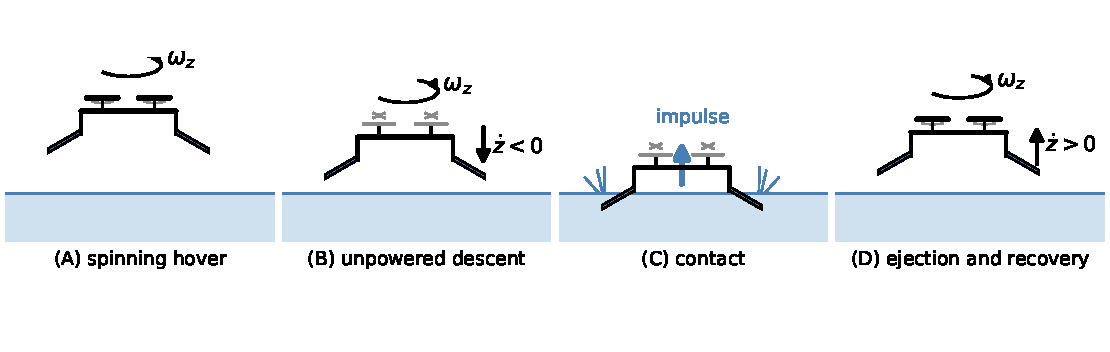
\includegraphics[width=\linewidth]{Assets/ch1fig1_hop_cycle.pdf}
    \caption{The hop cycle, in side view. \textbf{(A)} The vehicle hovers while spinning about its vertical axis at rate $\omega_z$: two rotors are mounted tangentially and drive the rotation, and two are mounted vertically and carry the lift. \textbf{(B)} The lift rotors are commanded to zero, marked by the crossed disks, and the vehicle descends unpowered; the tangential rotors keep driving the spin, so the hydrofoils reach the surface still sweeping at close to their hover speed. \textbf{(C)} The foils submerge and the water returns a large vertical impulse, braking the spin as it does so. \textbf{(D)} The vehicle leaves the surface climbing, control is restored, and the cycle repeats.}
    \label{fig:hop_cycle}
\end{figure}

\section{Related Work}
\label{sec:related_work}



\paragraph{Aquatic--aerial robots.}
Robots able to operate in both air and water have been pursued from several
directions.  One line of work develops fixed-wing vehicles that plunge into
the water and relaunch from it~\cite{siddall2014launching}, while another adapts rotorcraft to
land on, float on, or dive beneath the surface~\cite{alzubi2018loon}.  A third,
bio-inspired line mimics animals such as flying fish, diving birds, and
semi-aquatic insects that transition between swimming
and flight~\cite{zufferey2019consecutive,chen2017biologically}.

What these vehicles have in common is a difficulty of principle: the two media
make opposite demands of the same hardware.  Hydrodynamic loads at entry are
orders of magnitude larger than the aerodynamic loads the airframe is otherwise
sized for, so a structure light enough to fly must survive impacts it was not
built for.  A rotor sized to accelerate a large mass of air is badly matched to
water, which is dense enough to overload it at the same rotational speed.  And
everything that makes a vehicle amphibious, the sealing, the buoyancy, and the
structure that takes the impact, is mass the flight case carries for the whole
mission.  The usual resolution is to specialise, accepting reduced performance
in one medium or carrying a separate mechanism for the transition; in either
case water contact is treated as a destination, and the return to the air is
handled by restarting flight from rest or by a dedicated launch event.

\paragraph{Leaving the water.}
Departing the surface is the most demanding part of amphibious operation, and
the reason is a matter of scale.  The adhesive force holding a body to the
surface acts along the contact perimeter and therefore falls only linearly as
the vehicle is made smaller, while the thrust available to break it falls with
the disk area of the rotors; the ratio moves against the vehicle as it shrinks,
which is why the problem is acute at micro scale and mild at large scale.  A
departing vehicle must also accelerate the water entrained around it, adding
effective mass at precisely the moment it has none of the forward speed that
would otherwise generate lift.  It must therefore start from rest, in the worst
part of its thrust curve, against a force that does not scale in its favour.

Sustained motor power is the wrong instrument for this, and the reported
solutions all amount to releasing stored energy faster than the propulsion
system could deliver it: impulsive jumping~\cite{zufferey2019consecutive},
rapid gas generation or combustion~\cite{chen2017biologically}, or oversizing
the propulsion system so that its peak thrust suffices~\cite{alzubi2018loon}.
Each enables a transition, and each spends a large, non-recoverable share of
the energy budget doing so, which is what limits how many transitions a vehicle
can make.

\paragraph{Water-entry and skipping physics.}
The physics of objects bouncing on water has been studied independently of
robotics.  Stone-skipping and the related water-entry problem have been
analysed for both spinning and non-spinning bodies~\cite{bocquet2003physics,truscott2014water}, establishing
that a flat object striking water at a shallow angle experiences a large,
short-lived hydrodynamic reaction that can redirect it upward before it
sinks~\cite{clanet2004secrets}.

That reaction is inertial rather than buoyant.  During the contact the body
accelerates a mass of water downward and outward, and the force it feels is the
reaction to that momentum transfer; it grows with the square of the speed at
which the surface is swept and vanishes when the body is at rest.  Spin enters
this picture in two distinct ways, and the distinction matters for what
follows.  For a thrown stone, spin is stabilising: it holds the attack angle
against the torque of the impact, which would otherwise tumble the stone and
turn a skip into a splash~\cite{bocquet2003physics}.  For the vehicle described
here, spin instead supplies the sweep velocity itself, so the reaction is
available without the body having to travel horizontally across the surface at
all.  These studies characterise the conditions for a successful skip (approach
angle, speed, and spin) but consider passive, unpowered projectiles, and
neither role of spin has been examined for a controlled, self-propelled
vehicle.

\paragraph{Spinning multirotors.}
Multirotors that hover while spinning rapidly about their vertical axis have
been studied for some time, chiefly because a vehicle that gives up control of
its heading gains something in return.  Mueller and D'Andrea characterise
relaxed-hover solutions in which a multicopter sustains a constant spin rather
than holding a fixed heading, and show that abandoning yaw regulation is what
allows a quadrotor to keep flying after losing a
rotor~\cite{mueller2016relaxed}.  The SplitFlyer vehicles use the same freedom
differently, letting a quadrotor separate in flight into two bicopters, each
underactuated and able to fly only by
spinning~\cite{bai2020splitflyer,bai2022splitflyerair}.

Such vehicles are hard to control for two related reasons.  The first is that
the actuation axis rotates with the body, so a fixed differential thrust does
not produce a fixed torque in the inertial frame.  The command has to be
modulated in phase with the rotation, and any lag between measuring the yaw
angle and acting on it appears directly as an error in the direction of the
torque applied.  The second is that a body carrying large angular momentum
responds to a torque by precessing rather than by accelerating, so a torque
applied about one axis tilts the vehicle about the other, and the near-hover
intuition that roll torque produces roll no longer holds.  The standard
response is to stop describing the vehicle by its full orientation.  Yaw is
neither regulated nor of interest, only the direction of the thrust axis
matters, and that direction is a two-parameter object independent of the
instantaneous yaw angle; the gyroscopic reduced attitude dynamics written in
those two parameters are what make the problem
tractable~\cite{bai2022splitflyerair}.

In these platforms the
spin arises as a consequence of the actuator configuration: yaw torque cannot
be independently cancelled, and the vehicle settles at whatever rate balances
that residual torque.  The vehicle described here shares the fast-spin regime
and the reduced-attitude dynamics that come with it, but reaches it by different means: dedicated tangential rotors drive the rotation directly, so
the spin rate is commanded rather than inherited from the thrust balance.  This
matters because the hop depends on the tangential speed of the hydrofoils at
water contact: a spin rate that can be set is a design variable, not a
constraint to be worked around.

\paragraph{Summary.}
These bodies of work supply the individual ingredients (amphibious airframes, water-entry hydrodynamics, and control of fast-spinning multirotors) but none
combines them into a vehicle that uses spinning hydrofoils to hop repeatedly
across water, drawing the impulse that returns it to the air from the contact
itself rather than from a mechanism carried for the purpose.  That combination
is the subject of this thesis.

\section{Research Objectives}
\label{sec:research_objectives}

The goal of this thesis is to establish water-skipping as a practical mode of
locomotion for a micro aerial vehicle: to show that a small rotorcraft can
strike a water surface and be thrown back into the air by its own spinning
hydrofoils, and that it can do so repeatedly under closed-loop control.  This
goal breaks into four objectives.

\begin{enumerate}
  \item \textbf{Model the hop.}  Develop a quantitative model of the brief
    submersion phase that predicts the vertical impulse delivered to the
    vehicle as a function of the hydrofoil geometry, its attack angle, the spin
    rate at contact, and the descent velocity.  The model must be tractable
    enough to guide design decisions and to indicate which parameters dominate
    the outcome.

  \item \textbf{Design a vehicle that can survive and exploit the hop.}
    Realise an airframe that carries the hydrofoils at a useful radius, spins
    fast enough to give them the tangential speed the model requires, tolerates
    repeated water impact, and remains light enough to be ejected by the
    impulse its own foils generate.

  \item \textbf{Control a fast-spinning vehicle.}  Establish attitude and
    position control for an airframe rotating continuously about its vertical
    axis, where the spin dominates the attitude dynamics and the vehicle must
    be regulated as a rotating body rather than a heading-holding one.  The
    controller must hold station well enough to place the vehicle over a chosen
    point, execute a controlled descent onto the surface, and recover the
    vehicle after ejection.

  \item \textbf{Demonstrate the cycle experimentally.}  Show on hardware that
    the full sequence (hover, descend, contact, eject, recover) closes, and
    that the vehicle returns to controlled flight after water contact rather
    than merely surviving a single impact.
\end{enumerate}

\section{Thesis Contributions}
\label{sec:thesis_contributions}

The contributions of this thesis are as follows.

\begin{itemize}
  \item \textbf{A water-skipping locomotion mode for MAVs.}  The central
    contribution is the locomotion mode itself: a rotorcraft that hops across
    water on spinning hydrofoils, exploiting the density contrast between air
    and water so that the foils cost the vehicle little in flight yet deliver a
    large impulse during a contact lasting roughly a tenth of a second.  This treats
    water contact as a repeatable means of travel rather than as a landing, a
    dive, or a sampling stop.

  \item \textbf{A blade-element model of hydrofoil-driven ejection.}  A
    quasi-steady blade-element model of the submersion phase
    (Chapter~\ref{dynamic}) that predicts ejection velocity from foil geometry,
    attack angle, spin rate, and impact conditions, and identifies the
    parameters that govern whether a hop succeeds.

  \item \textbf{A spinning airframe with an independently commanded spin rate.}
    A vehicle design (Chapter~\ref{chapter:paperone}) in which two tangentially
    mounted rotors drive the rotation directly while two vertically mounted
    rotors provide lift and attitude authority.  Decoupling the spin from the
    lift channel turns the spin rate into a commanded design parameter, allowing
    the tangential blade speed at water contact to be set to what the hop
    requires.

  \item \textbf{Flight control at high spin rates.}  A control formulation and
    implementation (Chapter~\ref{chapter:papertwo}) that keeps the vehicle
    stable and position-controllable while spinning, together with an online
    method for separating the spin-synchronous artefact from the estimated
    attitude (Chapter~\ref{chapter:paperthree}).  In flight testing the vehicle
    remained controllable at spin rates approaching
    $10{,}000^{\circ}\,\mathrm{s^{-1}}$ without an upper limit being reached.

  \item \textbf{Experimental demonstration of repeated hops.}  Flight
    experiments (Chapter~\ref{chapter:paperthree}) demonstrating hops on a still
    water surface, including sequences in which the vehicle regains controlled
    flight after contact and returns toward its commanded height.
\end{itemize}

\section{Thesis Organization}

The remainder of this thesis is organized as follows:

\textbf{Chapter~\ref{dynamic}} develops the hydrodynamic model of the hop.  A
quasi-steady blade-element treatment of the submersion phase predicts the
forces generated by the hydrofoils as they sweep through the water, and
establishes how the resulting ejection depends on foil geometry, attack angle,
spin rate, and impact velocity.

\textbf{Chapter~\ref{chapter:paperone}} presents the design of the vehicle: the
airframe and its rotor configuration, the propulsion and power system, and the
geometry of the hydrofoils that carry out the hop.

\textbf{Chapter~\ref{chapter:papertwo}} develops the flight dynamics and
control of the spinning airframe, covering the coordinate frames and system
definition, the translational and attitude dynamics, the reduced dynamics that
apply under high yaw rate, and the controller built on them.

\textbf{Chapter~\ref{chapter:paperthree}} reports the experimental validation.
It describes the flight testing setup, an online method for separating
rotation-induced oscillations from the state estimate, and flight results for
constant-height jumping on water.

\textbf{Chapter~\ref{chapter:conclusion}} summarizes the contributions of this
thesis, discusses their implications, and outlines directions for future work.
